The given equation can be expressed as
\begin{align}
\label{eq:chapters/10/7/4/1vec}
    \myvec{2&1}\vec{x}&=4
\end{align}
Using section formula in
\eqref{eq:chapters/10/7/4/1vec},
\begin{align}
    \vec{n}^{\top}\myvec{\frac{k\vec{B+A}}{k+1}}&=c\\
    \implies k&=\frac{c-\vec{n}^{\top}\vec{A}}{\vec{n}^{\top}\vec{B}-c}
\end{align}
upon simplification.  Substituting numerical values, 
\begin{align}
    k=\frac{2}{9}
\end{align}
See 
\figref{fig:chapters/10/7/4/1vec}.
\begin{figure}[H]
\centering
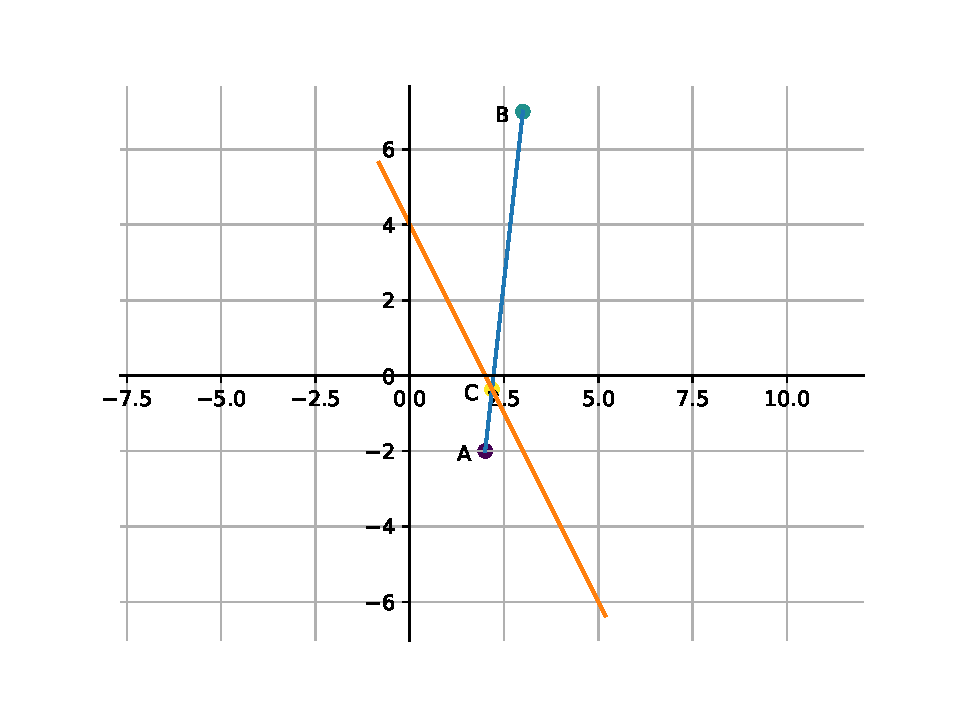
\includegraphics[width=0.75\columnwidth]{chapters/10/7/4/1/figs/fig.pdf}
\caption{}
\label{fig:chapters/10/7/4/1vec}
\end{figure}

